\documentclass{article}
\usepackage[a4paper,margin=1in]{geometry}
\usepackage{amsmath, amsfonts, amssymb, amstext, mathtools, stmaryrd, textcomp, xcolor, graphicx, tikz}
\usepackage[hidelinks]{hyperref}
\usetikzlibrary{automata, positioning, arrows, trees}
\tikzset{->,>=stealth,
every state/.style={thick, fill=gray!10}, 
initial text=$ $,
}
\newcommand{\answer}{\textcolor{red}}
\newcommand{\e}{\varepsilon}
\newcommand{\s}{\Sigma}
\newcommand{\g}{\Gamma}
\newcommand{\so}{\rightarrow}
\newcommand{\str}{\texttt}
\newcommand{\newp}{\\[2mm]}
\newcommand{\defeq}{\coloneqq}
\newcommand{\spc}{\textvisiblespace}

\title{Homework 07}
\author{Aaron Wang}
\date{April 11 2025}

\begin{document}
\maketitle
\begin{enumerate}
    \item \textbf{Bounds Checking}
    \begin{enumerate}
        \item [(a)] [Problem 5.30 (US ed. 5.14)] Prove that it is undecidable whether a Turing machine $M$, on input $w$, ever attempts to move its head past the left end of the tape.\newp
        
\textcolor{red}{
\begin{center}
\begin{minipage}{0.25\textwidth}
    i.
    \begin{center}
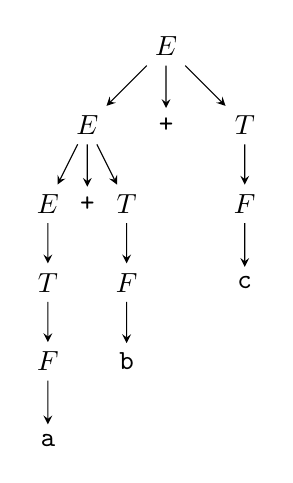
\begin{tikzpicture}[
    level distance=1cm,
    level 1/.style={sibling distance=1cm},
    level 2/.style={sibling distance=0.5cm}
]
    \node {$E$}
    child {node {$E$}
        child {node {$E$}
            child {node {$T$}
                child {node {$F$}
                    child {node {\str{a}}
                    }
                }
            }
        }
        child {node {\str{+}}}
        child {node {$T$}
            child {node {$F$}
                child {node {\str{b}}
                }
            }
        }
    }
    child {node {\str{+}}}
    child {node {$T$}
        child {node {$F$}
            child {node {\str{c}}}
        }
    };
\end{tikzpicture}
\end{center}
\end{minipage}
\begin{minipage}{0.25\textwidth}
    ii.
    \begin{center}
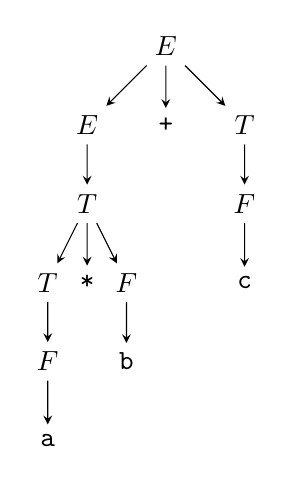
\begin{tikzpicture}[
    level distance=1cm,
    level 1/.style={sibling distance=1cm},
    level 2/.style={sibling distance=0.5cm}
]
    \node {$E$}
    child {node {$E$}
        child {node{$T$}
            child {node{$T$}
                child{node{$F$}
                    child{node{\str{a}}}
                }
            }
            child {node{\str{*}}}
            child {node{$F$}
                child{node {\str{b}}}
            }
        }
    }
    child {node {\str{+}}}
    child {node {$T$}
        child {node {$F$}
            child {node {\str{c}}}
        }
    };
\end{tikzpicture}
\end{center}
\end{minipage}
\begin{minipage}{0.25\textwidth}
    iii.
    \begin{center}
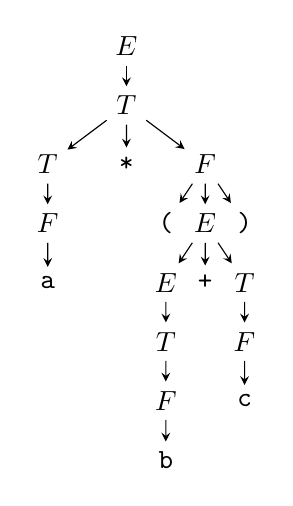
\begin{tikzpicture}[
    level distance=0.75cm,
    level 2/.style={sibling distance=1cm},
    level 3/.style={sibling distance=0.5cm}
]
    \node {$E$}
    child {node {$T$}
        child {node {$T$}
            child {node{$F$}
                child{node{\str{a}}}
            }
        }
        child {node {\str{*}}}
        child {node {$F$}
            child {node{\str{(}}}
            child {node {$E$}
                child {node {$E$}
                    child {node {$T$}
                        child {node{$F$}
                            child{node{\str{b}}}
                        }
                    }
                }
                child {node {\str{+}}}
                child {node {$T$}
                    child {node{$F$}
                        child{node{\str{c}}}
                    }
                }
            }
            child {node{\str{)}}}
        }
    };
\end{tikzpicture}
\end{center}
\end{minipage}
\end{center}
}

        \item [(b)]Prove that it is decidable whether a Turing machine $M$, on input $w$, ever attempts to move its head past the right end of the input string $w$. Your answer should be a high-level description of a TM.\newp
        \textcolor{red}{
\begin{align*}
& E \rightarrow E \: \str{+} \: T \: | \: T\\
& T \rightarrow T \: \str{*} \: F \: | \: F\\
& F \rightarrow O \: \str{$\uparrow$} \: F \: | \: O\\
& O \rightarrow \str{(}E\str{)} \: | \: \str{a} \: | \: \str{b} \: | \: \str{c}
\end{align*}
}
    \end{enumerate}
\newpage
    \item \textbf{\emph{The Power of 10}} is a set of rules for writing mission-critical code developed
at JPL.1 Let us call a Turing machine that complies with these rules \emph{10-compliant}. All that you need to know about 10-compliance is:
    \begin{itemize}
        \item A 10-compliant Turing machine always halts on every input
        \item It is decidable whether a Turing machine is 10-compliant.
    \end{itemize}
    In this problem, we’ll show that any such set of rules will be incomplete in the sense that there is a language $L_2$ that is decidable, yet no TM that decides $L_2$ complies with the rules.\newp
    Consider the language
    \[
        L_2 = \{\langle M \rangle | M\text{ is a 10-compliant TM that rejects } \langle M \rangle \}.
    \]
    \begin{enumerate}
        \item Prove that $L_2$ is decidable.\newp
        \begin{figure}[h]
\centering
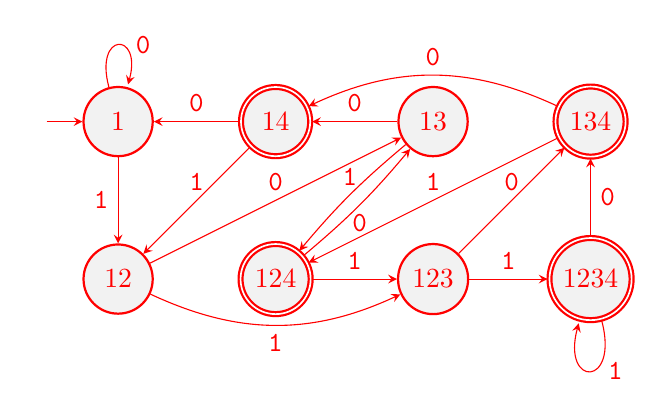
\begin{tikzpicture}
\color{red}
    % \node[state, initial] (q000) {$q_{000}$};
    % \node[state, yshift=-2cm] (q001) {$q_{001}$};
    % \node[state, xshift=4cm] (q010) {$q_{010}$};
    % \node[state, yshift=-2cm, xshift=4cm] (q011) {$q_{011}$};
    % \node[state, xshift=2cm, accepting] (q100) {$q_{100}$};
    % \node[state, yshift=-2cm, xshift=2cm, accepting] (q101) {$q_{101}$};
    % \node[state, xshift=6cm, accepting] (q110) {$q_{110}$};
    % \node[state, yshift=-2cm, xshift=6cm, accepting] (q111) {$q_{111}$};
    \node[state, initial] (q000) {1};
    \node[state, yshift=-2cm] (q001) {12};
    \node[state, xshift=4cm] (q010) {13};
    \node[state, yshift=-2cm, xshift=4cm] (q011) {123};
    \node[state, xshift=2cm, accepting] (q100) {14};
    \node[state, yshift=-2cm, xshift=2cm, accepting] (q101) {124};
    \node[state, xshift=6cm, accepting] (q110) {134};
    \node[state, yshift=-2cm, xshift=6cm, accepting] (q111) {1234};
    \draw 
        (q000) edge[loop above] node[right, xshift=1mm]{\str{0}} (q000)
        (q000) edge[] node[left]{\str{1}} (q001)
        (q001) edge[] node[above]{\str{0}} (q010)
        (q001) edge[bend right=25] node[below]{\str{1}} (q011)
        (q100) edge[] node[above]{\str{0}} (q000)
        (q100) edge[] node[above]{\str{1}} (q001)
        (q101) edge[bend right=5] node[below]{\str{0}} (q010)
        (q101) edge[] node[above]{\str{1}} (q011)
        (q010) edge[] node[above]{\str{0}} (q100)
        (q010) edge[bend right=5] node[above]{\str{1}} (q101)
        (q011) edge[] node[above]{\str{0}} (q110)
        (q011) edge[] node[above]{\str{1}} (q111)
        (q110) edge[bend right=25] node[above]{\str{0}} (q100)
        (q110) edge[] node[above]{\str{1}} (q101)
        (q111) edge[] node[right]{\str{0}} (q110)
        (q111) edge[loop below] node[right, xshift=1mm]{\str{1}} (q111)
    ;
\end{tikzpicture}
\end{figure}
        \item Prove that any TM that decides $L_2$ must not be 10-compliant.\newp
        \textcolor{red}{
    Proof: Assume $ADD$ is a regular language. Let $p$ be the pumping length from the Pumping Lemma. Let $s = \str{1}^p\str{=1}^p\str{+0}$. Observe that $s \in ADD$. The Pumping Lemma says that for some $xyz$, $s=xyz$, $|y| > 0$, $|xy| \leq p$ and $xyyz \in ADD$. Let $s' = xyyz$. Since $|xy| \leq p$, we know that $y$ contains all \str{1}s so $s' = \str{1}^r\str{=1}^p\str{+0}$ s.t. $r > p$. $s'$ is not true as  a number + 0 should be itself but it is not in this expression. Since $s'$ is not a true expression, $s' \notin ADD$ $\lightning$. Thus, by contradiction we have shown that $ADD$ can not be a regular language.
}
        \item Where in your solution to (a) is the violation of 10-compliance?\newp
        \textcolor{red}{
    This now accepts the string if \str{1} is the last, second-to-last, or third-to-last character.
}
    \end{enumerate}
\newpage
    \item \textbf{grep and sed}
    \begin{enumerate}
        \item [(a)] Prove that it is decidable whether two regular expressions are equivalent to each other. Hint: First prove that it is decidable whether a DFA recognizes the empty language. Then use closure properties.\newp
        \textcolor{red}{
    If $L$ is regular, we have an NFA without $\e$ transitions $N$ for $L$ s.t. $N = (Q, \s, \delta, s, F)$.\\
    Construct $N'= (Q', \s, \delta', s, F)$ to recognize STRETCH$(L)$\\
    \begin{enumerate}
        \item [1.]$Q'= Q \cup (\s_\e \times Q)$. This way we have the regular states and a state for every transition.
        \item [2.] $\s$ does not change.
        \item [3.] Define $\delta'$ so if $q$ is an original state ($q \in Q$), it will give transition state(s) and vice versa.
        \[
        \delta'\Big(q,a\Big)=  
        \begin{cases}
         (a,\delta(q,a)) & q \in Q  \\
         q_{\text{next(s)}}  & \text{s.t. } (a,q_{\text{next(s)}}) = q\\
         \emptyset & \text{otherwise}
        \end{cases}
        \]
        \item [4.] $s$ does not change.
        \item [5.] $F$ does not change.
    \end{enumerate}
    Let $L=\{\str{in},\str{out}\}$ as an example.\footnote{States without transitions were ommited from drawing}\\
    \begin{figure}[h]
\centering
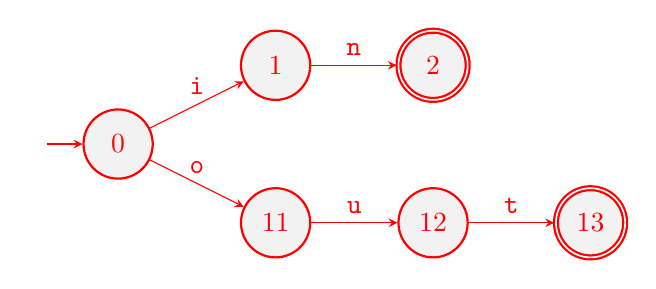
\begin{tikzpicture}
\color{red}
    \node[state, initial] (q0) {0};
    \node[state, xshift=2cm, yshift=1cm] (q1) {1};
    \node[state, xshift=4cm, yshift=1cm, accepting] (q2) {2};
    \node[state, xshift=2cm, yshift=-1cm] (q11) {11};
    \node[state, xshift=4cm, yshift=-1cm] (q12) {12};
    \node[state, xshift=6cm, yshift=-1cm, accepting] (q13) {13};
    
    \draw
    (q0) edge[] node[above]{\str{i}} (q1)
    (q1) edge[] node[above]{\str{n}} (q2)

    (q0) edge[] node[above]{\str{o}} (q11)
    (q11) edge[] node[above]{\str{u}} (q12)
    (q12) edge[] node[above]{\str{t}} (q13)
    ;
\end{tikzpicture}
\end{figure}\\
    STRETCH$(L)$
    \begin{figure}[h]
\centering
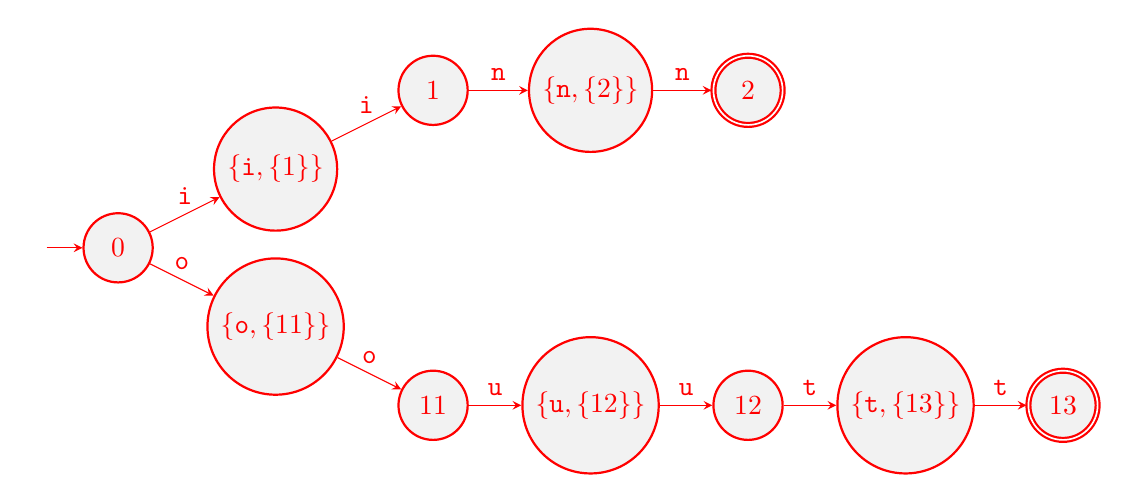
\begin{tikzpicture}
\color{red}
    \node[state, initial] (q0) {0};
    \node[state, xshift=2cm, yshift=1cm] (q1) {$\{\str{i},\{1\}\}$};
    \node[state, xshift=4cm, yshift=2cm] (q2) {1};
    \node[state, xshift=6cm, yshift=2cm] (q3) {$\{\str{n},\{2\}\}$};
    \node[state, xshift=8cm, yshift=2cm, accepting] (q4) {2};
    
    \node[state, xshift=2cm, yshift=-1cm] (q11) {$\{\str{o},\{11\}\}$};
    \node[state, xshift=4cm, yshift=-2cm] (q12) {11};
    \node[state, xshift=6cm, yshift=-2cm] (q13) {$\{\str{u},\{12\}\}$};
    \node[state, xshift=8cm, yshift=-2cm] (q14) {12};
    \node[state, xshift=10cm, yshift=-2cm] (q15) {$\{\str{t},\{13\}\}$};
    \node[state, xshift=12cm, yshift=-2cm, accepting] (q16) {13};
    
    \draw
    (q0) edge[] node[above]{\str{i}} (q1)
    (q1) edge[] node[above]{\str{i}} (q2)
    (q2) edge[] node[above]{\str{n}} (q3)
    (q3) edge[] node[above]{\str{n}} (q4)

    (q0) edge[] node[above]{\str{o}} (q11)
    (q11) edge[] node[above]{\str{o}} (q12)
    (q12) edge[] node[above]{\str{u}} (q13)
    (q13) edge[] node[above]{\str{u}} (q14)
    (q14) edge[] node[above]{\str{t}} (q15)
    (q15) edge[] node[above]{\str{t}} (q16)
    ;
\end{tikzpicture}
\end{figure}\\
    By proof of construction STRETCH$(L)$ is regular.
}
        \item [(b)] Prove that it is undecidable whether two \str{sed} programs (as defined in CP3) are equivalent to each other. Hint: Use CP3 Part 3.\newp
        \textcolor{red}{
    Proof: Assume $C$ is a regular language. Let $p$ be the pumping length from the Pumping Lemma. Let $s = \str{1}^p\str{01}^p$. Observe that $s \in C$. The Pumping Lemma says that for some $xyz$, $s=xyz$, $|y| > 0$, $|xy| \leq p$ and $xz \in C$. Let $s' = xz$. Since $|xy| \leq p$, we know that $y$ contains all \str{1}s so $s' = \str{1}^r\str{01}^p$ s.t. $r < p$. Thus $k \leq r$ and $w$ contains more than $p-1=r$ \str{1}s so $s' \notin L$ $\lightning$. Thus, by contradiction we have shown that $C$ can not be a regular language.
}
    \end{enumerate}
\end{enumerate}
\end{document}